%!TEX root = /Users/velrok/Dropbox/TheoInf Seminar/Ausarbeitung/Main.tex
\section{Ähnlichkeitstheorie} % (fold)
\label{sub:Aehnlichkeitstheorie}

Die Ähnlichkeitstheorie besagt, das sich die Eigenschaften einer Modal-Logik in der Relation der entsprechenden Kripkestrucktur widerspiegeln und vis versa. 
Dies schafft einen neuen Zugang zum Design von Modal-Logiken. 
In manchen Fällen mag es einfacher sein in den notwendigen Eigenschaften in Form von Formel-Schemata zu denken, in anderen ist es evtl. einfacher das Problem über die Relation zu verstehen. 
Im Folgenden wird gezeigt, wie die einzelnen Eigenschaften mit der Kripke-Struktur-Relation zusammen hängen.


\paragraph{Zusammenhang zwischen der Relation $R$ und den validen \formelSchemata}

Wir haben in \Abs{festlegung_von_attibuten_mit_R} den Zusammenhang zwischen der Transitivität von $R$ und der Validität der Formel \vierFormel durch die Intuition begründet, dass die \emph{positive Introspektion} gilt.
Es wird nun gezeigt, dass sich dieser Zusammenhang mathematisch beweisen lässt.
Dazu muss zunächst der Begriff \emph{Frame} eingeführt werden:

\begin{definition}
	\label{def:frame}
	Ein Frame $\Fancy{F} = (W,R)$ ist eine Menge von Welten $W$ und eine binäre Relation $R$ auf $W$.
	\cite[S.322]{huth2004logic}
\end{definition}

\emph{Frames} kann man sich also als \KS ohne \emph{Labeling-Funktion} vorstellen.
Damit beschreiben sie die selbe Struktur, jedoch unabhängig von der Konkreten Wissensbasis, sprich den geltenden Facken in jeder Welt.
Damit übernehmen sie in Kripke-Strukturen die selbe Rolle wie \formelSchemata in \MLFn .

\begin{definition}
	\label{def:frame_erfuellt}
	Ein Frame $\Fancy{F}$ erfüllt eine modal logische Formal $\psi$, wenn für jede \fachwort{Labelfunktion} $L: W \rightarrow \Fancy{P}(Atome)$ und jedes $w \in W$, es der Fall ist, dass $\Fancy{M},w \vDash \psi$ gilt. $\Fancy{M}$ ist das Model: $\Fancy{M} = (W,R,L)$.
	In diesem Falle schreiben wir $\Fancy{F} \vDash \psi$.
	\cite[S.322f]{huth2004logic}
\end{definition}

Wenn ein Frame eine Formel erfüllt erfüllt es auch das entsprechende Schema und umgekehrt \vglHuth{S.323}.

\begin{example}
	Das Beispiel-Frame auf \Abb{Kripke02} erfüllt die \TFormel.
	Um das zu beweisen muss man zeigen, dass jede Welt mit beliebiger Labeling-Funktion die Bedingung: wenn $x \VDash \Box p$ der Fall ist, dann gilt auch $x \VDash p$.
	Betrachten wie nun eine beliebige Welt $x \in W$ und setzen $x \VDash \Box p$, dann folgt aufgrund der Tatsache dass $R(x,x)$ gilt und der Regel für $\Box$ aus der \Def{reasoning}, dass $x \VDash p$ der Falls ein muss.
	Den $x$ zeigt auf sich selbst und ist damit in den von $x$ erreichbaren Welten enthalten

	\begin{figure}[h!]
		\label{fig:Kripke02}
		\centering
		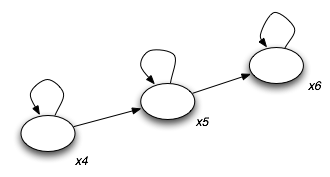
\includegraphics[width=10cm]{Images/Kripke02}
		\caption{Beispielframe}
	\end{figure}

	Da ein \emph{Frame} keine Annahme über eine konkrete Labeling-Funktion macht und wir gerade nachgewiesen haben, dass $\Box p \rightarrow p$ gilt, ist auch \TFormel der Fall.
	
	Die \vierFormel wird hingegen nicht erfüllt.
	Das Model in \Abb{Kripke03} beweist dies durch ein Gegenbeispiel
	\vglHuth{S.324f}.

	\begin{figure}[h!]
		\label{fig:Kripke03}
		\centering
		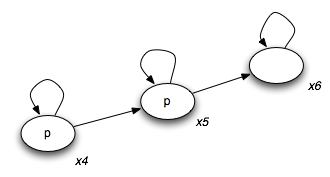
\includegraphics[width=10cm]{Images/Kripke03}
		\caption{Gegenbeispiel}
	\end{figure}

\end{example}

Auf Basis des Beispiels lässt sich folgendes Theorem aufstellen:

\begin{theorem}
	Gegeben ein Frame \FrameDef.
	\begin{enumerate}
		\item Die folgenden Aussagen sind äquvivalient:
		\begin{itemize}
			\item $R$ ist reflexiv
			\item $\Fancy{F}$ erfüllt \TFormel
			\item $\Fancy{F}$ erfüllt $\Box p \rightarrow p$
		\end{itemize} 
		
		\item Die folgenden Aussagen sind äquvivalient:
		\begin{itemize}
			\item $R$ ist transitiv
			\item $\Fancy{F}$ erfüllt \vierFormel
			\item $\Fancy{F}$ erfüllt $\Box p \rightarrow \Box \Box p$
		\end{itemize}
	\end{enumerate}
	\vglHuth{S.324f}.
\end{theorem}

\begin{proof}
	Um die Behauptungen zu beweisen wird ein Ring-Schluss geführt.\\
	Für jede Behauptung wird a) davon ausgegangen, dass $R$ die Eigenschaft besitzt und das daraus folgt, dass $\Fancy{F}$ das Schema erfüllt, b) das $\Fancy{F}$ das Schema erfüllt und daraus folgt, dass $\Fancy{F}$ auch die Formel-Instanz erfüllt und c) dass wenn $\Fancy{F}$ die Instanz erfüllt, dass $R$ die entsprechende Eigenschaft besitzt.
	
	\begin{enumerate}
		\item a) Gehen wir davon aus, dass $R$ reflexiv ist, $L$ eine Labeling-Funktion und \ModelDef ein Model der \NML. 
		Wir müssen zeigen das $\Fancy{M} \vDash \Box\phi \rightarrow \phi$ gilt. 
		Dies ist gleichbedeutend mit $x \Vdash \Box \phi \rightarrow \phi$ für alle Welten $x \in W$.
		Man beachte die Regel der Implikation in der \Def{reasoning}.
		Gehen wir also davon aus, das $x \Vdash \Box \phi$ der Fall ist, dann folgt aus der Regel für $\Box$ in \Def{reasoning} und der Tatsache das $R(x,x)$, dass $x \Vdash \phi$ zutrifft, womit dieser Schritt bewiesen ist.
		
		b) Es ist ausreichend für $\phi$ $p$ einzusetzen um dies zu zeigen.
		
		c) Gehen wir davon aus, dass das Framen $\Box p \rightarrow p$ erfüllt.
		Wir wollen zeigen, dass $R(x,x)$ dann ebenfalls gilt.\\
		Wir definieren die Label-Funktion $L$, so dass: $p \notin L(x)$ und $p \in L(y)$ für alle Welten $y$ außer $x$.\\
		\emph{Beweis durch Wiederspruch}. Gehen wir davon aus $R(x,x)$ gilt nicht.
		Dann gilt $x \Vdash \Box p$ weil alle Welten außer $x$ $p$ erfüllen.
		Da aber $\Fancy{F}$ $\Box p \rightarrow p$ erfüllt ergibt sich $x \Vdash p$.
		Das ist ein Wiederspruch zu der Annahme, das $R(x,x)$ nicht gilt.
		In der Folge muss $R(x,x)$ der Fall sein.
		
		\item a) Gehen wir davon aus, dass $R$ transitiv ist, $L$ eine Labeling-Funktion und \ModelDef ein Model der \NML. 
		Wir müssen zeigen das $\Fancy{M} \vDash \Box \phi \rightarrow \Box \Box \phi$ gilt. 
		Dies ist gleichbedeutend mit $x \Vdash \Box \phi \rightarrow \Box \Box \phi$ für alle Welten $x \in W$.\\
		Nehmen wir an $x \Vdash \Box \phi$ gilt so müssen wir zeigen dass auch $x \Vdash \Box \Box \phi$ gilt. 
		Nach der Regel $\Box$ nach der \Def{reasoning} ist dies der Fall, wenn $y \Vdash \Box \phi$ für alle $R(x,y)$, was wiederum der Fall ist wenn $z \Vdash \phi$ für alle $R(y,z)$ gilt.
		Nemen wir also an es gäbe $y$ und $z$, sodass $R(x,y)$ und $R(y,z)$.
		Weil $R$ transitiv ist wissen wir das es auch $R(x,z)$ gibt.
		Nach der Voraussetzung $x \Vdash \Box \phi$ und $R(x,z)$ gilt also $z \Vdash \phi$, was nachzuweisen war.
		
		b) Wir setzen wieder für $\phi$ $p$ ein und sind fertig.
		
		c) Gehen wir davon aus, dass das Framen $\Box p \rightarrow \Box \Box p$ erfüllt.
		Wir wollen zeigen, dass wenn $R(x,y)$ und $R(y,z)$ gilt $R(x,z)$ der Fall sein muss.\\
		Wir definieren die Label-Funktion $L$, so dass: $p \notin L(z)$ und $p \in L(w)$ für alle Welten $w$ außer $z$.\\
		\emph{Beweis durch Wiederspruch}. Gehen wir davon aus $R(x,z)$ sei nicht der Fall.
		Dann gilt $x \Vdash \Box p$, denn alle Welten $w$ außer $z$ erfüllen $p$.
		Aus dem Axion $\Box p \rightarrow \Box \Box p$ folgt $x \Vdash \Box \Box p$, woraus folgt $y \Vdash \Box p$ woraus nach $R(y,z)$ $z \Vdash p$ was der Annahme widerspricht.
		Weshalb $R(x,z)$ der Fall sein muss.
	\end{enumerate}
	\vglHuth{S.324f}
\end{proof}

Die Tabelle \Tab{attributesIncludingR} vervollständigt die Zusammenhänge zwischen \formelSchemata und Relationseigenschaften.

\begin{theorem}
	Ein \emph{Frame} \FrameDef erfüllt ein \formelSchema in \Tab{attributesIncludingR} gdw. $R$ die entsprechende Eigenschaft aufweist. \citeHuth{S.325}
\end{theorem}

\begin{table}[h!]
	\centering
	\label{tab:attributesIncludingR}
	\begin{tabular}{cll}
	\hline
	\hline
	Name & Formel Schema\\
	\hline
	T & $\Box \phi \rightarrow \phi$									&	reflexiv\\
	B & $\phi \rightarrow \Box \Diamond\phi$					& symmetrisch\\
	D & $\Box \phi \rightarrow \Diamond \phi$					& seriell\\
	4 & $\Box \phi \rightarrow \Box \Box \phi$				& transitiv\\
	5 & $\Diamond \phi \rightarrow \Box \Diamond \phi$& euklidisch\\
	  & $\Box \phi \leftrightarrow \Diamond \phi$			& funktional\\
	  & $\Box(\phi \wedge \Box \phi \rightarrow \psi) \vee \Box(\psi \wedge \Box \psi \rightarrow \phi)$& vorwärts funktional\\
	\hline
	\end{tabular}\\
	\caption{Attribut Bezeichnungen und entsprechende \formelSchemata so wie $R$ Eigenschaften.\\Quelle: \citeHuth[S.325]}
\end{table}






% subsection Aehnlichkeitstheorie (end)
